\documentclass{beamer}

\usepackage{graphicx}
\usepackage{algorithm2e}
\usepackage{textpos}
\usepackage{etoolbox}
\usepackage{verbatim}

\setbeamertemplate{caption}[numbered]

\usepackage{tikz}
\usetikzlibrary{shapes.geometric}
\usetikzlibrary{arrows,shapes,trees}
\usetikzlibrary{calc,shapes.multipart,chains,arrows}
\usetikzlibrary{matrix,positioning}

\usepackage[dvipsnames]{xcolor}
\definecolor{pblue}{rgb}{0.13,0.13,1}
\definecolor{pgreen}{rgb}{0,0.5,0}
\definecolor{pred}{rgb}{0.9,0,0}
\definecolor{pgrey}{rgb}{0.46,0.45,0.48}

\usepackage{listings}
\lstset{language=Java,
    showspaces=false,
    showtabs=false,
    breaklines=true,
    showstringspaces=false,
    breakatwhitespace=true,
    commentstyle=\color{pgreen},
    keywordstyle=\color{pblue},
    stringstyle=\color{pred},
    basicstyle=\footnotesize,
    colframe=white!75!black,
    moredelim=[is][\textcolor{pgrey}]{\%\%}{\%\%}
}

\pgfdeclareshape{plain triangle}{
    \nodeparts{}
    \anchor{center}{\pgfpoint{0cm}{0cm}}
    \behindbackgroundpath{
		\path [draw,dashed] (0,0) -- (.5,-1) -- (-0.5,-1) -- cycle;
   }
   \pgfsetcolor{red}
}

\pgfdeclareshape{blue triangle}{
    \nodeparts{}
    \anchor{center}{\pgfpoint{0cm}{0cm}}
    \behindbackgroundpath{
		\path [draw,dashed, fill=blue] (0,0) -- (.5,-1) -- (-0.5,-1) -- cycle;
   }
   \pgfsetcolor{red}
}

\pgfdeclareshape{red triangle}{
    \nodeparts{}
    \anchor{center}{\pgfpoint{0cm}{0cm}}
    \behindbackgroundpath{
		\path [draw,dashed, fill=red] (0,0) -- (.5,-1) -- (-0.5,-1) -- cycle;
   }
   \pgfsetcolor{red}
}
\usetheme{Madrid}
\useoutertheme{miniframes} % Alternatively: miniframes, infolines, split



% Setup the university's color pallette
\definecolor{UIUCorange}{RGB}{19, 41, 75} % UBC Blue (primary)
\definecolor{UIUCblue}{RGB}{232, 74, 39} % UBC Grey (secondary)


\setbeamercolor{palette primary}{bg=UIUCorange,fg=white}
\setbeamercolor{palette secondary}{bg=UIUCblue,fg=white}
\setbeamercolor{palette tertiary}{bg=UIUCblue,fg=white}
\setbeamercolor{palette quaternary}{bg=UIUCblue,fg=white}
\setbeamercolor{structure}{fg=UIUCorange} % itemize, enumerate, etc
\setbeamercolor{section in toc}{fg=UIUCblue} % TOC sections

\setbeamercolor{subsection in head/foot}{bg=UIUCorange,fg=UIUCblue}
\setbeamercolor{subsection in head/foot}{bg=UIUCorange,fg=UIUCblue}

\usepackage[utf8]{inputenc}


%Information to be included in the title page:
\title{\textbf{Graphs Continued}}
%\author{\textbf{David H Smith IV}}
%\institute[\textbf{UIUC}]{\textbf{University of Illinois Urbana-Champaign}}
%\date{\textbf{}}
\documentclass{beamer}


\usepackage{graphicx}
\usepackage{algorithm2e}
\usepackage{textpos}
\usepackage{etoolbox}
\usepackage{verbatim}

\setbeamertemplate{caption}[numbered]

\usepackage{tikz}
\usetikzlibrary{shapes.geometric}
\usetikzlibrary{arrows,shapes,trees}
\usetikzlibrary{calc,shapes.multipart,chains,arrows}
\usetikzlibrary{matrix,positioning}

\usepackage[dvipsnames]{xcolor}
\definecolor{pblue}{rgb}{0.13,0.13,1}
\definecolor{pgreen}{rgb}{0,0.5,0}
\definecolor{pred}{rgb}{0.9,0,0}
\definecolor{pgrey}{rgb}{0.46,0.45,0.48}

\usepackage{listings}
\lstset{language=Java,
    showspaces=false,
    showtabs=false,
    breaklines=true,
    showstringspaces=false,
    breakatwhitespace=true,
    commentstyle=\color{pgreen},
    keywordstyle=\color{pblue},
    stringstyle=\color{pred},
    basicstyle=\footnotesize,
    colframe=white!75!black,
    moredelim=[is][\textcolor{pgrey}]{\%\%}{\%\%}
}

\pgfdeclareshape{plain triangle}{
    \nodeparts{}
    \anchor{center}{\pgfpoint{0cm}{0cm}}
    \behindbackgroundpath{
		\path [draw,dashed] (0,0) -- (.5,-1) -- (-0.5,-1) -- cycle;
   }
   \pgfsetcolor{red}
}

\pgfdeclareshape{blue triangle}{
    \nodeparts{}
    \anchor{center}{\pgfpoint{0cm}{0cm}}
    \behindbackgroundpath{
		\path [draw,dashed, fill=blue] (0,0) -- (.5,-1) -- (-0.5,-1) -- cycle;
   }
   \pgfsetcolor{red}
}

\pgfdeclareshape{red triangle}{
    \nodeparts{}
    \anchor{center}{\pgfpoint{0cm}{0cm}}
    \behindbackgroundpath{
		\path [draw,dashed, fill=red] (0,0) -- (.5,-1) -- (-0.5,-1) -- cycle;
   }
   \pgfsetcolor{red}
}
\usetheme{Madrid}
\useoutertheme{miniframes} % Alternatively: miniframes, infolines, split

\setbeamertemplate{title page}[default][colsep=-4bp,rounded=true]
\addtobeamertemplate{title page}{\vspace{3\baselineskip}}{}
\addtobeamertemplate{title page}{
    \begin{textblock*}{\paperwidth}(-1.0em, -1.2em)
        \includegraphics[width=\paperwidth, height=\paperheight]{imgs/uiuc.jpg}
    \end{textblock*} 
}{}



% Setup the university's color pallette
\definecolor{UIUCorange}{RGB}{19, 41, 75} % UBC Blue (primary)
\definecolor{UIUCblue}{RGB}{232, 74, 39} % UBC Grey (secondary)


\setbeamercolor{palette primary}{bg=UIUCorange,fg=white}
\setbeamercolor{palette secondary}{bg=UIUCblue,fg=white}
\setbeamercolor{palette tertiary}{bg=UIUCblue,fg=white}
\setbeamercolor{palette quaternary}{bg=UIUCblue,fg=white}
\setbeamercolor{structure}{fg=UIUCorange} % itemize, enumerate, etc
\setbeamercolor{section in toc}{fg=UIUCblue} % TOC sections

\setbeamercolor{subsection in head/foot}{bg=UIUCorange,fg=UIUCblue}
\setbeamercolor{subsection in head/foot}{bg=UIUCorange,fg=UIUCblue}

\usepackage[utf8]{inputenc}

\begin{document}

\frame{\titlepage}

\section{Adj. Matrix Drawbacks}

\begin{frame}[fragile]
    \frametitle{Adj. Matrix - Disadvantages}
    \centering
    \begin{minipage}{0.49\textwidth}
    \resizebox{!}{0.89\textwidth}{
    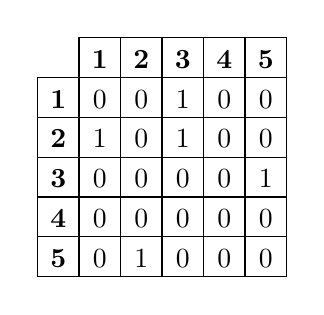
\begin{tikzpicture}[Bullet/.style={circle,draw,fill=black,inner sep=1.5pt},
        adjacency matrix/.style={ampersand replacement=\&,matrix of math nodes,
        row 1/.append style={nodes={font=\boldmath}},
        column 1/.append style={nodes={font=\boldmath}},nodes in empty cells,
        nodes={draw,minimum width=1.5em,text height=1.8ex},column sep=-\pgflinewidth,row
        sep=-\pgflinewidth}]

    \def\adjancymatrix{%
        {
            {0, 0, 4, 0,  0}, %
            {5, 0,  3, 0,  0}, %
            {0, 0,  0, 0,  2}, %
            {0, 0,  0, 0,  0}, %
            {0, 1,  0, 0,  0}
        }
    } 

    \let\mymatrixcontent\empty
    \def\mymatrixcontent{|[draw=none]|\& 1 \& 2 \& 3 \& 4 \& 5\\}
    \begin{scope}[local bounding box=right,xshift=10cm]
        %\foreach \X in {1,...,3}
        %{
        %    \node[draw, circle] (E\X) at (90+72-\X*72:2) {$v_\X$} ;
        %}
        %\node[draw, circle] (E5) at (90+72-4*72:2) {$v_5$} ; 
        %\node[draw, circle] (E4) at (90+72-5*72:2) {$v_4$} ; 
        \foreach \X in {1,...,5}
        {\begingroup\edef\x{\endgroup
            \noexpand\gappto\noexpand\mymatrixcontent{\X }}\x
            \foreach \Y in {1,...,5}
            {\pgfmathtruncatemacro{\itest}{\adjancymatrix[\X-1][\Y-1]}
                \ifnum\itest=0
                    \begingroup\edef\x{\endgroup
                    \noexpand\gappto\noexpand\mymatrixcontent{\& 0}}\x
                \else
                    %\draw[->] (E\X) edge node[align=left, fill=white, line width=2pt] {\itest} (E\Y);
                    \begingroup\edef\x{\endgroup
                    \noexpand\gappto\noexpand\mymatrixcontent{\& 1}}\x
                \fi
            }
            \gappto\mymatrixcontent{\\}
        }
    \end{scope} 
    \matrix (rightmat) [below=of right,adjacency matrix]{
        \mymatrixcontent
    };
    \end{tikzpicture}}
    \end{minipage}
    \begin{minipage}{0.49\textwidth}
        \begin{enumerate}
            \item \textbf{Space Complexity: } $O(V^2)$
            \item We have to resize the 2d array everytime we create or delete a vertex (like arraylist).
        \end{enumerate}
    \end{minipage}
\end{frame}

\section{Adj. List}

\begin{frame}[fragile]
    \frametitle{Graphs are a Collection of Vertecies and Edges}
    \begin{minipage}{0.49\textwidth}
	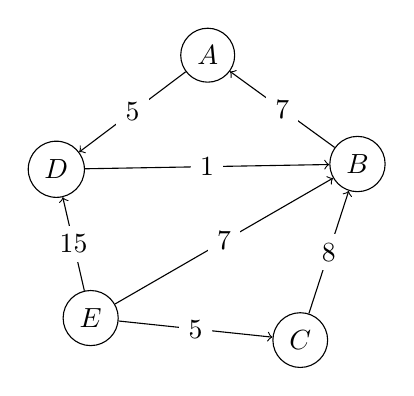
\begin{tikzpicture}[Bullet/.style={circle,draw,fill=black,inner sep=1.5pt},
		adjacency matrix/.style={ampersand replacement=\&,matrix of math nodes,
		row 1/.append style={nodes={font=\boldmath}},
		column 1/.append style={nodes={font=\boldmath}},nodes in empty cells,
		nodes={draw,minimum width=1.5em,text height=1.8ex},column sep=-\pgflinewidth,row
		sep=-\pgflinewidth}]

	\def\adjancymatrix{%
		{
            {0,0,0,5,0},%
            {7,0,0,0,0},%
            {0,8,0,0,0},%
            {0,1,0,0,0},%
            {0,7,5,15,0}
        }
    } 

	%\let\mymatrixcontent\empty
	%\def\mymatrixcontent{|[draw=none]|\& 1 \& 2 \& 3 \& 4 \& 5\\}
	\begin{scope}[local bounding box=right,xshift=10cm]
        \node[draw, circle] (E1) at (90+72-72:2) {$A$} ;
        \node[draw, circle] (E2) at (90+72-2*72:2) {$B$} ;
        \node[draw, circle] (E3) at (90+72-3*72:2) {$C$} ;
		\node[draw, circle] (E4) at (1100+72-4*72:2) {$D$} ; 
		\node[draw, circle] (E5) at (150+72-5*72:2) {$E$} ; 
		\foreach \X in {1,...,5}
		{\begingroup\edef\x{\endgroup
			\noexpand\gappto\noexpand\mymatrixcontent{\X }}\x
			\foreach \Y in {1,...,5}
			{\pgfmathtruncatemacro{\itest}{\adjancymatrix[\X-1][\Y-1]}
				\ifnum\itest=0
					\begingroup\edef\x{\endgroup
					\noexpand\gappto\noexpand\mymatrixcontent{\& \itest }}\x
				\else
                    \path[->] (E\X) edge node[align=left, fill=white] {\itest} (E\Y);
					\begingroup\edef\x{\endgroup
					\noexpand\gappto\noexpand\mymatrixcontent{\& \itest }}\x
				\fi
			}
			\gappto\mymatrixcontent{\\}
		}
	\end{scope} 
	%\matrix (rightmat) [right=of right,adjacency matrix]{
	%	\mymatrixcontent
	%};
    \end{tikzpicture}
    \end{minipage}
    \hfill
    \begin{minipage}{0.49\textwidth}
        Recall, a graph is: \[G = (V, E)\]
        \textbf{Vertecies ($V$): }$A,\  B,\ C,\ D,\ E$ \\
        \textbf{Edges ($E$)}
        \begin{itemize}
            \item $ A \rightarrow  D $, 5
            \item $ B \rightarrow  A $, 7
            \item $ C \rightarrow  B $, 8
            \item $ D \rightarrow  B $, 1
            \item $ E \rightarrow  D $, 15
            \item $ E \rightarrow  B $, 7
            \item $ E \rightarrow  C $, 5
        \end{itemize}
    \end{minipage}
    \centering
    \vfill
\end{frame}

\begin{frame}[fragile]
    \frametitle{Graph - Adj List Representation}
    \begin{minipage}{0.49\textwidth}
        Recall, a graph is: \[G = (V, E)\]
        \textbf{Vertecies ($V$): }$A,\  B,\ C,\ D,\ E$ \\
        \textbf{Edges ($E$)}
        \begin{itemize}
            \item $ A \rightarrow  D $, 5
            \item $ B \rightarrow  A $, 7
            \item $ C \rightarrow  B $, 8
            \item $ D \rightarrow  B $, 1
            \item $ E \rightarrow  D $, 15
            \item $ E \rightarrow  B $, 7
            \item $ E \rightarrow  C $, 5
        \end{itemize}
    \end{minipage}
    \begin{minipage}{0.49\textwidth}
    \resizebox{\textwidth}{!}{
        \begin{figure}[H]
    \centering
    \begin{tikzpicture}[list/.style={rectangle split, rectangle split parts=2, draw, rectangle split verical}, start chain]

            \node[list,on chain] (A) {value=12 \nodepart{second} weight=1};

    \end{tikzpicture}\\
    \caption{A visual representation of an edge}
    \label{fig:edge}
\end{figure}

Our implementation of an adjacency list will be composed of a HashMap with
vertices as keys and edge lists as values. As you will see in
Section~\ref{sec:edge}, an edge is composed of two attributes, a weight and the
vertex containing a destination (Figure~\ref{fig:edge}). The following is an
example of how a graph is represented by an adjacency matrix.\\

\begin{minipage}{0.4\textwidth}
    {\renewcommand{\arraystretch}{1.2}% for the vertical padding}
    \begin{tabular}{| c | l |}
        \hline
        Key & Value \\
        \hline
        a & \rule[11.2ex]{0pt}{0pt}  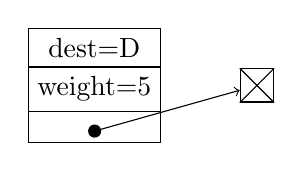
\begin{tikzpicture}[list/.style={rectangle split, rectangle split parts=3, draw}, start chain]

                \foreach \x/ \w in {D/5}{
                    \node[list,on chain] (\x) {dest=\x \nodepart{second} weight=\w};
                }


                \node[on chain,draw,inner sep=6pt] (N) {};
                \draw (N.north east) -- (N.south west);
                \draw (N.north west) -- (N.south east);


                \foreach \s/ \d in {D/N}{
                    \draw[*->] let \p1 = (\s.three), \p2 = (\s.three) in (\x1,\y2) -- (\d);
                }

        \end{tikzpicture}
        \\ \hline
        b & \rule[11.2ex]{0pt}{0pt} 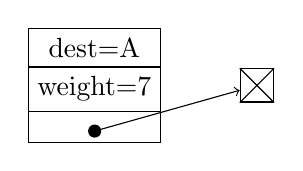
\begin{tikzpicture}[list/.style={rectangle split, rectangle split parts=3, draw}, start chain]

                \foreach \x/ \w in {A/7}{
                    \node[list,on chain] (\x) {dest=\x \nodepart{second} weight=\w};
                }


                \node[on chain,draw,inner sep=6pt] (N) {};
                \draw (N.north east) -- (N.south west);
                \draw (N.north west) -- (N.south east);


                \foreach \s/ \d in {A/N}{
                    \draw[*->] let \p1 = (\s.three), \p2 = (\s.three) in (\x1,\y2) -- (\d);
                }

        \end{tikzpicture}
        \\ \hline
        c & \rule[11.2ex]{0pt}{0pt} 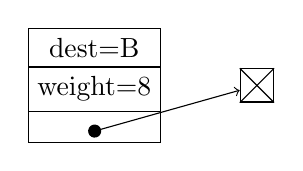
\begin{tikzpicture}[list/.style={rectangle split, rectangle split parts=3, draw}, start chain]

                \foreach \x/ \w in {B/8}{
                    \node[list,on chain] (\x) {dest=\x \nodepart{second} weight=\w};
                }


                \node[on chain,draw,inner sep=6pt] (N) {};
                \draw (N.north east) -- (N.south west);
                \draw (N.north west) -- (N.south east);


                \foreach \s/ \d in {B/N}{
                    \draw[*->] let \p1 = (\s.three), \p2 = (\s.three) in (\x1,\y2) -- (\d);
                }
        \end{tikzpicture}
        \\ \hline
        d & \rule[11.2ex]{0pt}{0pt} 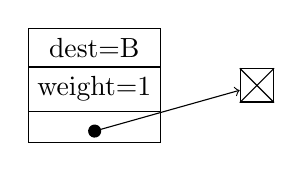
\begin{tikzpicture}[list/.style={rectangle split, rectangle split parts=3, draw}, start chain]

                \foreach \x/ \w in {B/1}{
                    \node[list,on chain] (\x) {dest=\x \nodepart{second} weight=\w};
                }


                \node[on chain,draw,inner sep=6pt] (N) {};
                \draw (N.north east) -- (N.south west);
                \draw (N.north west) -- (N.south east);


                \foreach \s/ \d in {B/N}{
                    \draw[*->] let \p1 = (\s.three), \p2 = (\s.three) in (\x1,\y2) -- (\d);
                }

        \end{tikzpicture}
        \\ \hline
        e & \rule[11.2ex]{0pt}{0pt} 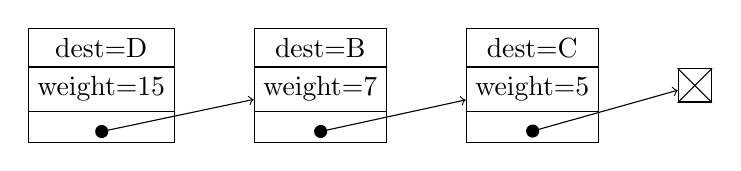
\begin{tikzpicture}[list/.style={rectangle split, rectangle split parts=3, draw}, start chain]

                \foreach \x/ \w in {D/15, B/7, C/5}{
                    \node[list,on chain] (\x) {dest=\x \nodepart{second} weight=\w};
                }


                \node[on chain,draw,inner sep=6pt] (N) {};
                \draw (N.north east) -- (N.south west);
                \draw (N.north west) -- (N.south east);


                \foreach \s/ \d in {D/B, B/C, C/N}{
                    \draw[*->] let \p1 = (\s.three), \p2 = (\s.three) in (\x1,\y2) -- (\d);
                }



        \end{tikzpicture}
        \\ \hline

    \end{tabular}
    }
\end{minipage}
\hfill
\begin{minipage}{0.4\textwidth}
\begin{figure}[H]
\centering
\begin{tikzpicture}[scale=0.7, auto,swap]

    \node[starting vertex] (a) at (-5,2) {a};
    \foreach \pos/\name in {{(-2,5)/b}, {(2,2)/c},
                            {(-3,-2)/d}, {(0,0)/e}}
        \node[vertex] (\name) at \pos {$\name$};

    \foreach \source/ \dest/ \weight in {b/a/7, c/b/8,a/d/5,
                                         e/b/7, e/c/5,e/d/15,
                                         d/b/1
                                         }
        \draw[-{>},line width=0.9pt] (\source) -- node[weight] {$\weight$} (\dest);
\end{tikzpicture}
\end{figure}
\end{minipage}

\\
\vspace{0.25cm}

    }
\end{minipage}
\end{frame}

\begin{frame}[fragile]
    \frametitle{Adjacency List}
    \centering
    \resizebox{0.49\textwidth}{!}{
        \begin{figure}[H]
    \centering
    \begin{tikzpicture}[list/.style={rectangle split, rectangle split parts=2, draw, rectangle split verical}, start chain]

            \node[list,on chain] (A) {value=12 \nodepart{second} weight=1};

    \end{tikzpicture}\\
    \caption{A visual representation of an edge}
    \label{fig:edge}
\end{figure}

Our implementation of an adjacency list will be composed of a HashMap with
vertices as keys and edge lists as values. As you will see in
Section~\ref{sec:edge}, an edge is composed of two attributes, a weight and the
vertex containing a destination (Figure~\ref{fig:edge}). The following is an
example of how a graph is represented by an adjacency matrix.\\

\begin{minipage}{0.4\textwidth}
    {\renewcommand{\arraystretch}{1.2}% for the vertical padding}
    \begin{tabular}{| c | l |}
        \hline
        Key & Value \\
        \hline
        a & \rule[11.2ex]{0pt}{0pt}  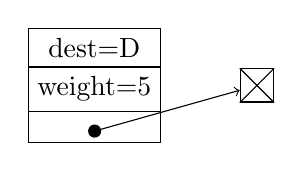
\begin{tikzpicture}[list/.style={rectangle split, rectangle split parts=3, draw}, start chain]

                \foreach \x/ \w in {D/5}{
                    \node[list,on chain] (\x) {dest=\x \nodepart{second} weight=\w};
                }


                \node[on chain,draw,inner sep=6pt] (N) {};
                \draw (N.north east) -- (N.south west);
                \draw (N.north west) -- (N.south east);


                \foreach \s/ \d in {D/N}{
                    \draw[*->] let \p1 = (\s.three), \p2 = (\s.three) in (\x1,\y2) -- (\d);
                }

        \end{tikzpicture}
        \\ \hline
        b & \rule[11.2ex]{0pt}{0pt} 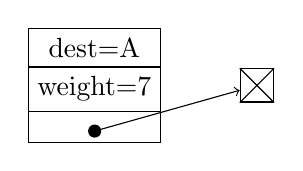
\begin{tikzpicture}[list/.style={rectangle split, rectangle split parts=3, draw}, start chain]

                \foreach \x/ \w in {A/7}{
                    \node[list,on chain] (\x) {dest=\x \nodepart{second} weight=\w};
                }


                \node[on chain,draw,inner sep=6pt] (N) {};
                \draw (N.north east) -- (N.south west);
                \draw (N.north west) -- (N.south east);


                \foreach \s/ \d in {A/N}{
                    \draw[*->] let \p1 = (\s.three), \p2 = (\s.three) in (\x1,\y2) -- (\d);
                }

        \end{tikzpicture}
        \\ \hline
        c & \rule[11.2ex]{0pt}{0pt} 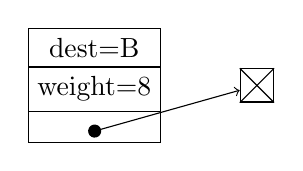
\begin{tikzpicture}[list/.style={rectangle split, rectangle split parts=3, draw}, start chain]

                \foreach \x/ \w in {B/8}{
                    \node[list,on chain] (\x) {dest=\x \nodepart{second} weight=\w};
                }


                \node[on chain,draw,inner sep=6pt] (N) {};
                \draw (N.north east) -- (N.south west);
                \draw (N.north west) -- (N.south east);


                \foreach \s/ \d in {B/N}{
                    \draw[*->] let \p1 = (\s.three), \p2 = (\s.three) in (\x1,\y2) -- (\d);
                }
        \end{tikzpicture}
        \\ \hline
        d & \rule[11.2ex]{0pt}{0pt} 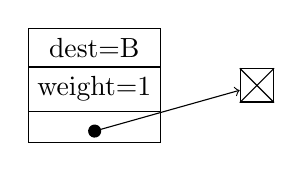
\begin{tikzpicture}[list/.style={rectangle split, rectangle split parts=3, draw}, start chain]

                \foreach \x/ \w in {B/1}{
                    \node[list,on chain] (\x) {dest=\x \nodepart{second} weight=\w};
                }


                \node[on chain,draw,inner sep=6pt] (N) {};
                \draw (N.north east) -- (N.south west);
                \draw (N.north west) -- (N.south east);


                \foreach \s/ \d in {B/N}{
                    \draw[*->] let \p1 = (\s.three), \p2 = (\s.three) in (\x1,\y2) -- (\d);
                }

        \end{tikzpicture}
        \\ \hline
        e & \rule[11.2ex]{0pt}{0pt} 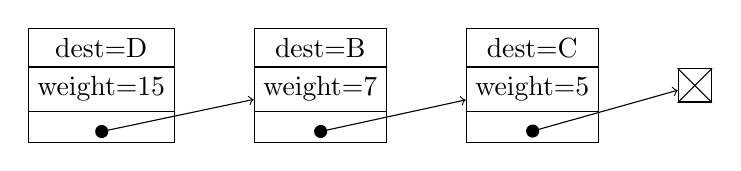
\begin{tikzpicture}[list/.style={rectangle split, rectangle split parts=3, draw}, start chain]

                \foreach \x/ \w in {D/15, B/7, C/5}{
                    \node[list,on chain] (\x) {dest=\x \nodepart{second} weight=\w};
                }


                \node[on chain,draw,inner sep=6pt] (N) {};
                \draw (N.north east) -- (N.south west);
                \draw (N.north west) -- (N.south east);


                \foreach \s/ \d in {D/B, B/C, C/N}{
                    \draw[*->] let \p1 = (\s.three), \p2 = (\s.three) in (\x1,\y2) -- (\d);
                }



        \end{tikzpicture}
        \\ \hline

    \end{tabular}
    }
\end{minipage}
\hfill
\begin{minipage}{0.4\textwidth}
\begin{figure}[H]
\centering
\begin{tikzpicture}[scale=0.7, auto,swap]

    \node[starting vertex] (a) at (-5,2) {a};
    \foreach \pos/\name in {{(-2,5)/b}, {(2,2)/c},
                            {(-3,-2)/d}, {(0,0)/e}}
        \node[vertex] (\name) at \pos {$\name$};

    \foreach \source/ \dest/ \weight in {b/a/7, c/b/8,a/d/5,
                                         e/b/7, e/c/5,e/d/15,
                                         d/b/1
                                         }
        \draw[-{>},line width=0.9pt] (\source) -- node[weight] {$\weight$} (\dest);
\end{tikzpicture}
\end{figure}
\end{minipage}

\\
\vspace{0.25cm}

    }
    \vfill\\
    \hspace{1.5cm}
    \begin{minipage}{0.70\textwidth}
    \begin{lstlisting}[basicstyle=\tiny, frame=trBL]
    private Map<String, List<Edge>> map = new HashMap<>();
    \end{lstlisting}
    \end{minipage}
\end{frame}

\section{Edge Class}

\begin{frame}[fragile]
    \frametitle{Activity - Constructing the Edge Class}
    \begin{enumerate}
        \item For the adjacency list we will be creating lists of edges to associate with vertecies
        \item Construct an Edge class in the worksheet with the following attributes
            \begin{itemize}
                \item Two \lstinline|private final| attributes: 1) a string for the destination and 2) a integer for the weight.
                \item Getters for both of those attributes.
            \end{itemize}
    \end{enumerate}
\end{frame}

\section{Adding Vertecies}

\begin{frame}[fragile]
    \frametitle{Algorithm - Adding Vertecies}
    \begin{minipage}{0.49\textwidth}
        \centering
        \resizebox{0.7\textwidth}{!}{
            \input{./imgs/adj-addvertex-1.tex}
        }
        \vspace{.5cm}\\
        \tiny
        \textbf{Step 1: Have an Adj List}
    \end{minipage}
    \begin{minipage}{0.49\textwidth}
        \centering
        \resizebox{0.7\textwidth}{!}{
            \input{./imgs/adj-addvertex-2.tex}
        }
        \vspace{.5cm}\\
        \tiny
        \textbf{Step 2: After Adding the ``Z'' Vertex and a list to store its edges.}
    \end{minipage}
    \vfill\\
    \hspace{4cm}
    \begin{minipage}{0.35\textwidth}
    \begin{lstlisting}[basicstyle=\tiny, frame=trBL]
map.containsKey(key);
map.put(key, val);
map.putIfAbsent(key, val);
    \end{lstlisting}
    \end{minipage}
\end{frame}

\section{Adding Edges}

\begin{frame}[fragile]
    \frametitle{Algorithm - Adding Directed Edges}
    \begin{minipage}{0.49\textwidth}
        \centering
        \resizebox{0.7\textwidth}{!}{
            \input{./imgs/adj-addedge1.tex}
        }
        \vspace{0.5cm}\\
        \tiny
        \textbf{Step 1:} Get the list associated with the source vertex. Lets use \texttt{C} as an example.
    \end{minipage}
    \begin{minipage}{0.49\textwidth}
        \centering
        \resizebox{0.7\textwidth}{!}{
            \input{./imgs/adj-addedge2.tex}
        }
        \vspace{0.5cm}\\
        \tiny
        \textbf{Step 2:} Add the edge to the end of that list. In this case, one to A with a weight of 2.
    \end{minipage}
    \vfill\\
    \hspace{4cm}
    \begin{minipage}{0.30\textwidth}
    \begin{lstlisting}[basicstyle=\tiny, frame=trBL]
map.get(key);
    \end{lstlisting}
    \end{minipage}
\end{frame}

\section{Removing Edges}

\begin{frame}[fragile]
    \frametitle{Algorithm - Removing Edges}
    \centering
    \resizebox{0.49\textwidth}{!}{
        {\renewcommand{\arraystretch}{1.2}% for the vertical padding}
\begin{tabular}{| c | l |}
    \hline
    Key & Value \\
    \hline
    A & \rule[11.2ex]{0pt}{0pt}  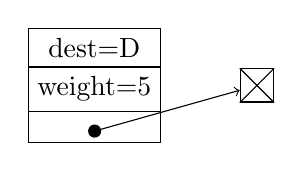
\begin{tikzpicture}[list/.style={rectangle split, rectangle split parts=3, draw}, start chain]

            \foreach \x/ \w in {D/5}{
                \node[list,on chain] (\x) {dest=\x \nodepart{second} weight=\w};
            }


            \node[on chain,draw,inner sep=6pt] (N) {};
            \draw (N.north east) -- (N.south west);
            \draw (N.north west) -- (N.south east);


            \foreach \s/ \d in {D/N}{
                \draw[*->] let \p1 = (\s.three), \p2 = (\s.three) in (\x1,\y2) -- (\d);
            }

    \end{tikzpicture}
    \\ \hline
    B & \rule[11.2ex]{0pt}{0pt} 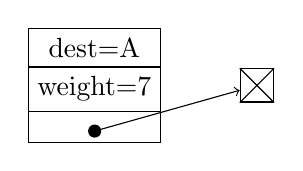
\begin{tikzpicture}[list/.style={rectangle split, rectangle split parts=3, draw}, start chain]

            \foreach \x/ \w in {A/7}{
                \node[list,on chain] (\x) {dest=\x \nodepart{second} weight=\w};
            }


            \node[on chain,draw,inner sep=6pt] (N) {};
            \draw (N.north east) -- (N.south west);
            \draw (N.north west) -- (N.south east);


            \foreach \s/ \d in {A/N}{
                \draw[*->] let \p1 = (\s.three), \p2 = (\s.three) in (\x1,\y2) -- (\d);
            }

    \end{tikzpicture}
    \\ \hline
    C & \rule[11.2ex]{0pt}{0pt} 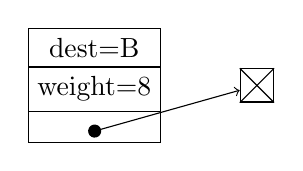
\begin{tikzpicture}[list/.style={rectangle split, rectangle split parts=3, draw}, start chain]

            \foreach \x/ \w in {B/8}{
                \node[list,on chain] (\x) {dest=\x \nodepart{second} weight=\w};
            }


            \node[on chain,draw,inner sep=6pt] (N) {};
            \draw (N.north east) -- (N.south west);
            \draw (N.north west) -- (N.south east);


            \foreach \s/ \d in {B/N}{
                \draw[*->] let \p1 = (\s.three), \p2 = (\s.three) in (\x1,\y2) -- (\d);
            }
    \end{tikzpicture}
    \\ \hline
    D & \rule[11.2ex]{0pt}{0pt} 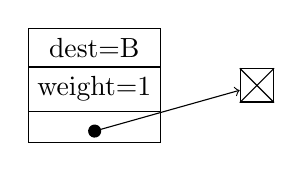
\begin{tikzpicture}[list/.style={rectangle split, rectangle split parts=3, draw}, start chain]
            \foreach \x/ \w in {B/1}{
                \node[list,on chain] (\x) {dest=\x \nodepart{second} weight=\w};
            }


            \node[on chain,draw,inner sep=6pt] (N) {};
            \draw (N.north east) -- (N.south west);
            \draw (N.north west) -- (N.south east);


            \foreach \s/ \d in {B/N}{
                \draw[*->] let \p1 = (\s.three), \p2 = (\s.three) in (\x1,\y2) -- (\d);
            }


    \end{tikzpicture}
    \\ \hline
    \textcolor{red}{\textbf{E}} & \rule[11.2ex]{0pt}{0pt} 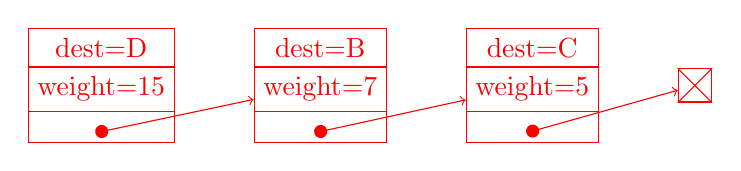
\begin{tikzpicture}[color=red, list/.style={rectangle split, rectangle split parts=3, draw}, start chain]

            \foreach \x/ \w in {D/15, B/7, C/5}{
                \node[list,on chain] (\x) {dest=\x \nodepart{second} weight=\w};
            }


            \node[on chain,draw,inner sep=6pt] (N) {};
            \draw (N.north east) -- (N.south west);
            \draw (N.north west) -- (N.south east);


            \foreach \s/ \d in {D/B, B/C, C/N}{
                \draw[*->] let \p1 = (\s.three), \p2 = (\s.three) in (\x1,\y2) -- (\d);
            }



    \end{tikzpicture}
    \\ \hline

\end{tabular}
}



    }
    \vfill\\
    \textbf{Step 1: Get the list associated with the source of the edge you want to remove. For example E.}
\end{frame}

\begin{frame}[fragile]
    \frametitle{Algorithm - Removing Edges}
    \centering
    \resizebox{0.49\textwidth}{!}{
        \input{./imgs/adj-remove2.tex}
    }
    \vfill\\
    \textbf{Step 2: Iterate over the list to get the index of the Edge object with the matching destination. If we want to remove B, that would be index 1.}
\end{frame}

\begin{frame}[fragile]
    \frametitle{Algorithm - Removing Edges}
    \centering
    \resizebox{0.39\textwidth}{!}{
        \input{./imgs/adj-remove3.tex}
    }
    \vfill\\
    \textbf{Step 3: Remove the element at that index from the list.}
\end{frame}

\begin{frame}[fragile]
    \frametitle{Activity - Constructing a Digraph}
    \textbf{Go to the worksheet and implement the Digraph class with the algorithms we just went over.}
\end{frame}



\end{document}
